\documentclass{article}
\usepackage[utf8]{inputenc}

\title{Transfer Learning, Residual Connections, and Inception Modules}
\author{Justin Zhang}
\date{December 2017}


\usepackage[letterpaper, margin=1in]{geometry}
\usepackage{natbib}
\usepackage{graphicx}
\usepackage{amsmath}

\begin{document}

\maketitle

\section{Introduction}
We have learned a lot about image classification and using convolutional neural networks for a host of problems. However, we also know that training all of these structures takes a lot of time and computational power we don't have. So how can we utilize these structures?

\section{ImageNet}

One of the greatest problems in AI has been in working with images and visual input. As we learned before, convolutional neural networks are very effective at doing this. One of the great challenges that has pushed this field forward is ImageNet. ImageNet is a classification challenge where 1 million images are given and must be classified. Many groups all over the world strive to improve modern AI technology in order to top the charts annually. In order to produce more successful results, many optimizations have been done to the standard neural network.

It turns out that training on ImageNet is quite useful. Since ImageNet contains a very large variety of classes and labels, it's not only a comprehensive computer vision benchmark. It can be hypothesized that the features learned at the very lowest of levels are simple, generalizable features that are actually not problem specific, a result that is empirically demonstrated: if these networks are trained to learn additional classes, they converge much faster than random weight initialization.



\section{Transferring Knowledge}
How is this useful? In humans, if we see a new object we try to describe it certain terms we already know, using things such as smooth, red, etc. In the same regard, neural networks can transfer over generic image-based knowledge to new patterns. By using the weights that other organizations have trained and obtained on ImageNet, we can have a baseline that already gives us the core image analysis power needed. This knowledge can easily be exploited by us! In fact, many modern machine learning libraries such as Keras already have several common models such as VGG, ResNet, and Inception newtorks built in for transfer learning.

\section{Applying Our Data}
In general, the process for transfer learning is pretty straightforward. We take the weights, and instead of randomly initializing, we use the pretrained weights and begin from there. We then run as normal. However, often this is either too slow or we don't have enough data. In that case, we do something called freezing. When layers are ``frozen", their weights won't change throughout backpropagation. A common approach is to freeze the convolutional layers, which learn generally about images, and add on or retrain the top portion consisting of fully connected layers. This way, we can use transfer learning as a method to go from an image to some extracted features we can train on. If the data isn't very similar for our transferred task, we have enough computational power, and we have enough data, we then would unfreeze the lower layers to allow the convolutional layers to fine-tune.

The learning rate and learning rate decay should be kept relatively small throughout the fine-tuning process. This allows transfer learning to make subtle changes to the weights to account for the change in tasks.

It should be noted that the correspondence between the small features that make up the image (the ``style" of an image) and earlier convolutional layers, as well as the correspondence between the content of the image and the later dense layers, is illustrated nicely with style transfer networks, or networks that transfer the style of one image with another's content. The interested reader should read up on this for more intuition on transfer learning.

\section{Softmax}
\begin{center}
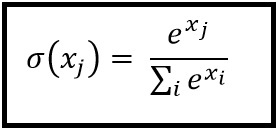
\includegraphics[scale=0.5]{softmax}
\end{center}
\subsection{Definition}
So how specifically do we encode class probabilities in a network? Normally, in a two-class scenario, we can have one neuron at the end with the sigmoid activation. Recall the sigmoid function maps values between zero and one, allowing us to treat this value as a probability.

In cases where there's more than one class, at the end of the network, we have one neuron per each output class. ImageNet allows you to take your top five best guesses since many classes turn out to be similar (say different breeds of dogs). We want a way to estimate the probability of each label. To do this, we use the softmax layer. This function essentially takes the sum of all the outputs and raises it to $e$ to make it positive. It then calculates the probability of each label by taking its value raised to $e$ over the total sum just calculated, which gives the fraction of a given class in the total sum. We can treat this as a probability.

The softmax classifier can be measured in similarity to a correct distribution with an information theory concept of cross-entropy, defined as:
$$ H(p, q) = -\sum_x p(x)\log q(x)$$.

For a ``true" distribution $p$ and a predicted distribution $q$, this compares the two. Note that $p$, in image classification, will be a one-hot vector (i.e. [0,0,0, ..., 0, 1, 0, ..., 0]). Thus, our final measure for the network's correctness is:

$$ L = - \log(\sigma) $$ where $\sigma$ is the correct class's probability.

This is the negative log-likelihood, and can be used as a loss function for softmax. Consider why: if a probability is near $0$, our loss value will be very high. Alternatively, a value near $1$ will give us a loss value near $0$.

To do back-propagation, we can simply apply chain rule. The equation is given below:

$$ \frac{dL}{dx_i} = \frac{dL}{d\sigma} \frac{d\sigma}{dx_i} $$
$$ \frac{dL}{dx_i} = -\frac{1}{\sigma}\frac{(e^{x_i}\sum_j e^{x_j}-e^{2x_i})}{(\sum_j e^{x_j})^2} $$

We obtain the second equation with the quotient rule.

\section{Residual Connections}
\begin{center}
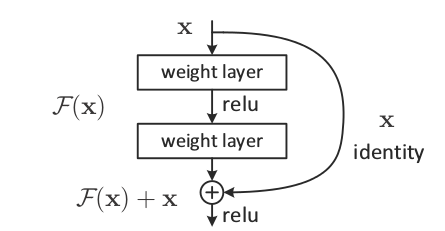
\includegraphics[scale=0.5]{resnet}
\end{center}
\subsection{Definition}
For some years, the trend in machine learning was always adding more layers. With the constant improvement in GPUs, if something didn't work now, the solution was to wait a year and add more layers. However, one big issue that exists with this is the vanishing gradient. At some point, the connection between the input and the output is too spaced away and the network can no longer learn significant features at the lower layers (the degredation problem). However, we know that deeper networks can learn more complex features more easily and are much better suited to handle hard problems. To solve this, researchers produced residual connections. Residual connections are essentially these nodes which consist of a set of layers. Each node extracts some features from the raw image and then combines this information with the original input to pass into the subsequent layer. In this way, features can be extracted in depth and subsequent layers can maintain access to the original information. 

\begin{center}
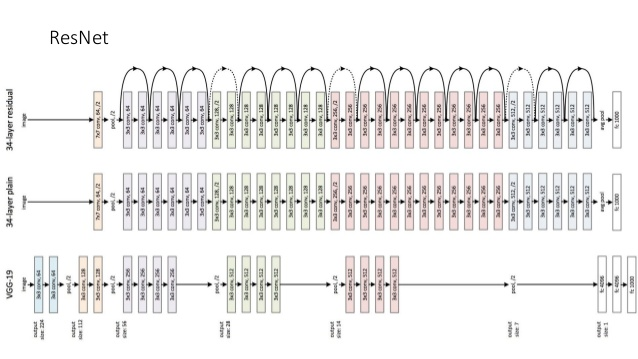
\includegraphics[scale=0.5]{resnet.jpg}
\end{center}
\subsection{Definition}
As you can see, ResNet allows for much greater depth compared to VGG. The image above is the smallest conventional size of ResNet. Typical applications use ResNet-50 at least and high-end ones use ResNet-152. The sheer power of these structures has allowed for 92.9 percent accuracy on ImageNet and the usage of training on fancy GPUs with lots of data.

Formally, let's look at residual connections in-depth.
The goal in training ResNets are for the nonlinearities to learn $F(x) := H(x) - x$, where $H(x)$ is the desired underlying mapping. Then, as you can see in the diagram,  we add $x$ with the residual connection to obtain $H(x)$.

There are a number of observations you should note about shortcut connections (the ones that do identity mappings).
\begin{enumerate}
    \item They do not add extra parameters, and thus no extra computational complexity.
    \item ResNets can easily be trained with regular methods (SGD).
    \item Since nonlinearities are universal approximators, clearly the residual unit is also a universal approximator.
    \item The ResNet is (theoretically) no harder to train than equivalent networks with only the identity connections (no non-linearities between them). This is because, if necessary, gradient solvers can drive the nonlinearities to zero to only, in effect, use the identity connection (this won't be the case in practical use, however, rendering the residual unit beneficial).
\end{enumerate}

\subsection{Some math}
Note that you don't need to know the content in this section to apply ResNet.

As portrayed in the figure under ``Residual Connections", the block is defined as:
$$ y = F(x; W_i) + x$$
where
$$ F = W_2 \sigma(W_1 x) $$
and $\sigma$ is the ReLU activation.

Of course, the dimensions of $x$ and $F$ may be different. Thus we can perform a linear projection $W_s$ on $x$:

$$ y = F(x; W_i) + W_s x$$, where $W_s$ is a square matrix. This is sufficient and cheap to solve the degradation problem. Other methods (zero-padding, for instance) can also work. The empirical differences of these methods is very small.

Empirically, $F$ should have 2-3 layers; more are possible, but only 1 has no observed benefits.

Clearly $y$ is defined by a differentiable operation (addition) on two differentable terms. Thus $y$ can be back-propagated through and trained. The advantages of defining $y$ are listed in the previous section.

\section{Inception}
\begin{center}
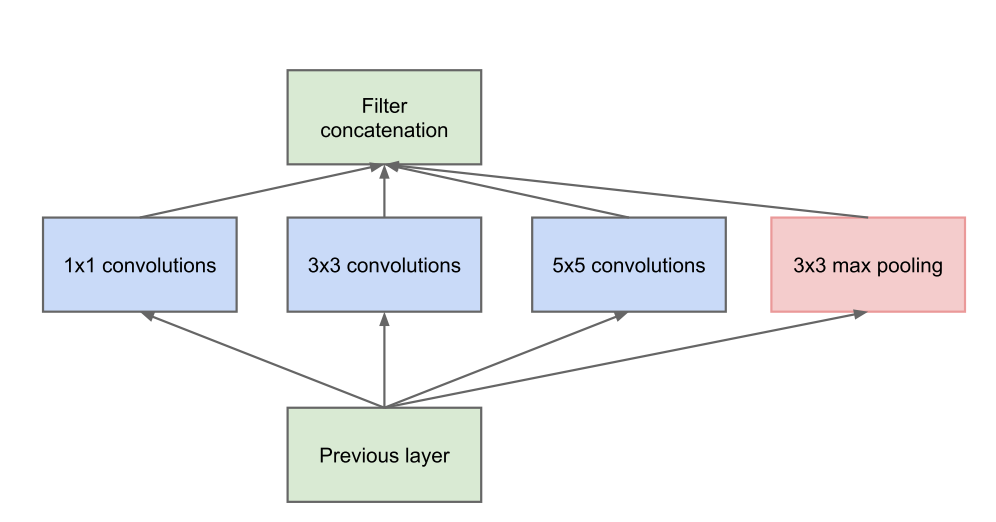
\includegraphics[scale=0.5]{inception}
\end{center}
\subsection{Definition}
The next major improvement in recent years in image classification has been in the usage of multiple parallel layers in each residual node. Each of these sets of layers, as seen in the image above, contains different filter sizes, allowing for a varying size of features to be extracted. From this, each residual node can learn much more and increased information can be packed in. This has culminated in Inception-ResNet structures capable of producing results more accurate than humans on image classification.

\subsection{Specifics}
    The idea of Inception layers was based off the ``we need to go deeper" internet meme. This automatically gives it more legitimacy over general neural networks, which were modeled after the brain, and reinforcement learning, which was modeled after operant conditioning.
    
    ``Deeper," in this context, refers to two things: a new level of network organization and literal deeper networks. 
    
    To understand the Inception architecture, consider a fundamental trade-off of convolutional networks: the most straightforward way to improve performance is to increase network size. This comes with two drawbacks: overfitting (due to more parameters) and a large drop in performance. Sparsely connected architectures could theoretically solve this as well as better approximate biological processes and single out discrimanatory features, but technical details prevent modern computers from efficiently doing numerical computations with sparse matrices.
    
    The Inception architecture seeks to use varying filter sizes (allowing the model to choose the optimal one, or even combine them) while trying to mimic the result of a sparse structure. 
    
    \begin{center}
    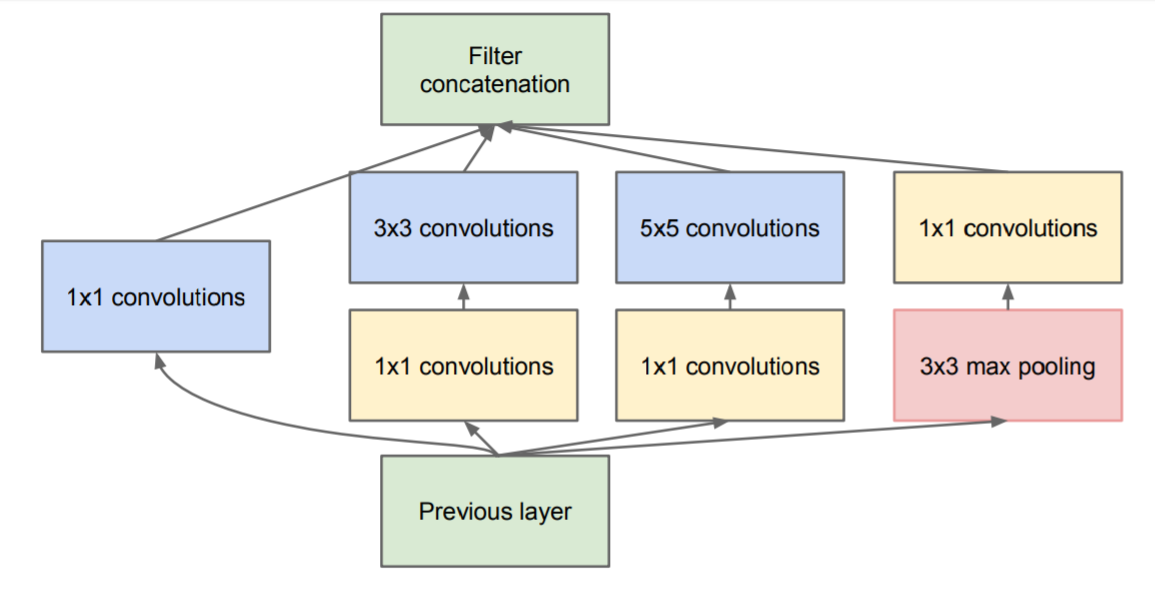
\includegraphics[scale=0.5]{inception2}
    \end{center}
    
    This revised architecture uses dimensionality reduction to make the inception module more efficient and to keep representations of data sparse (i.e. dense convolutions are used with sparser data). Specifically, max pooling (for obvious reasons) and 1x1 convolutions are used.
    
    These 1x1 convolutions do the following:
    \begin{enumerate}
        \item Make the network deeper
        \item Reduce dimensions (the number of feature maps)
        \item Add more non-linearities (ReLU after the 1x1 convolutions)
    \end{enumerate}
    
    Generally, Inception modules are only used in the beginning of a convolutional network, for memory efficiency. 
    
    

\section{To the Future}
In large part, following these advances, image classification has improved a lot. However, especially with the advent of adversarial examples for mainstream convolutional neural networks, the process clearly isn't perfect, or even close to the way humans perceive objects. Thus there is still much research to be done in more closely mimicking the way people identify objects.


\end{document}
